% Numerical reference is the manuscript summary in experiments_final/04_Total_Summary.
% Figures use the manuscript reference and final physical experiment summaries.
\subsection{System Evaluation}~\label{exp:sys_eval}

\begin{table*}[t]
\centering
\caption{Query timing and query selection strategies. Columns indicate query timing criteria and rows indicate query selection criteria. KnowNo and IntroPlan and Query-Action are the baselines. Fully-Random and Q1--Q2 and W1--W3 are the ablation configurations. Ours serves as the reference method for both comparisons. A dash denotes a combination not evaluated in this study.}
\label{tab:query_strategy_matrix}
\small
\newcommand{\queryhighlight}[2]{%
    \tikz[baseline=(marker.base)]{%
        \node[inner xsep=3pt,inner ysep=1pt] (marker) {\phantom{#2}};
        \fill[#1,opacity=0.7]
            ([xshift=-1pt,yshift=-0.5pt]marker.south west) --
            ([xshift=1pt,yshift=0.5pt]marker.south east) --
            ([xshift=2pt,yshift=-0.5pt]marker.north east) --
            ([xshift=0.5pt,yshift=0.5pt]marker.north west) -- cycle;
        \node[inner xsep=3pt,inner ysep=1pt] at (marker.center) {#2};
    }%
}
\begin{tabular}{lcccc}
\toprule
\shortstack{When $\rightarrow$\\What $\downarrow$} & Random & Conformal Prediction & Reward-based & Confidence \\
\midrule
Random & \queryhighlight{blue!25}{Fully-Random} & -- & -- & \queryhighlight{blue!25}{Q1} \\
Conformal Set & -- & \queryhighlight{yellow!65}{KnowNo, IntroPlan} & -- & -- \\
Reward-based & -- & -- & \queryhighlight{yellow!65}{Query-Action} & \queryhighlight{blue!25}{Q2} \\
Entropy Gain & \queryhighlight{blue!25}{W1} & \queryhighlight{blue!25}{W2} & \queryhighlight{blue!25}{W3} & \queryhighlight{green!35}{\textbf{Ours}} \\
\bottomrule
\end{tabular}
\end{table*}

Table~\ref{tab:query_strategy_matrix} summarizes the baseline and ablation configurations. The baseline comparison in Sec.~\ref{exp:sys_baseline} evaluates KnowNo, IntroPlan, and Query-Action against Ours. The baseline evaluation covers oracle responses in simulation and VLM and human responses during physical execution. The ablation study in Sec.~\ref{exp:policy_ablation} evaluates Fully-Random, Q1--Q2, and W1--W3 against Ours where W1--W3 examine query timing (when) and Q1--Q2 examine query selection (what). Finally the threshold study in Sec.~\ref{exp:sys_threshold} examines how the confidence threshold affects task success and query count. Both the ablation and threshold studies use oracle responses in simulation.



\subsubsection{Baseline Comparison}~\label{exp:sys_baseline}

\noindent\textbf{Oracle}. The oracle comparison includes three baselines with the query timing and selection strategies summarized in Table~\ref{tab:query_strategy_matrix}. KnowNo~\cite{ren2023robots} requests an action choice if its conformal prediction set does not specify a single ordinary action. IntroPlan~\cite{liang2024introspective} extends KnowNo and incorporates retrieved examples and explanations into candidate evaluation before it requests an action choice. Query-Action follows the standard POMDP approach to information gathering~\cite{kaelbling1998planning}. It includes Boolean state queries in the POMCP action space and selects them according to expected cumulative reward. Table~\ref{tab:baseline_results} and Fig.~\ref{fig:baseline_results} compare the four methods. 

\begin{figure*}[!tp]
\centering
\begin{subfigure}[t]{0.247\textwidth}
\centering
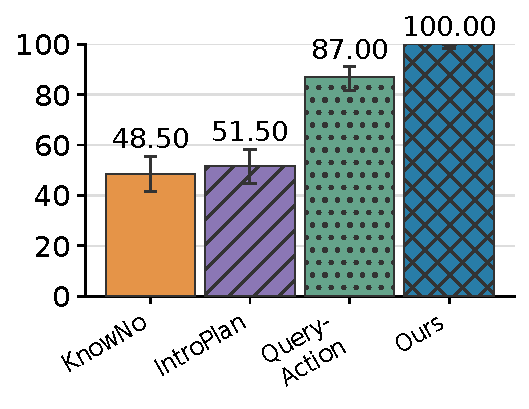
\includegraphics[width=\linewidth,height=.16\textheight,keepaspectratio]{figures/exp_oracle_waste_success.pdf}
\caption{WasteSorting\\Success rate (\%).}
\label{fig:baseline_oracle_waste_success}
\end{subfigure}%
\hspace{0.004\textwidth}%
\begin{subfigure}[t]{0.247\textwidth}
\centering
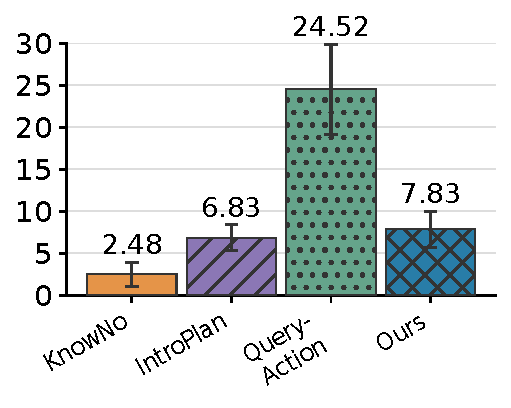
\includegraphics[width=\linewidth,height=.16\textheight,keepaspectratio]{figures/exp_oracle_waste_queries.pdf}
\caption{WasteSorting\\Query count.}
\label{fig:baseline_oracle_waste_queries}
\end{subfigure}%
\hspace{0.004\textwidth}%
\begin{subfigure}[t]{0.247\textwidth}
\centering
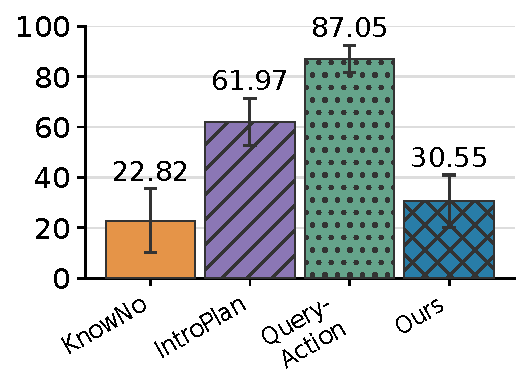
\includegraphics[width=\linewidth,height=.16\textheight,keepaspectratio]{figures/exp_oracle_waste_query_probability.pdf}
\caption{WasteSorting\\Query probability (\%).}
\label{fig:baseline_oracle_waste_query_probability}
\end{subfigure}%
\hspace{0.004\textwidth}%
\begin{subfigure}[t]{0.247\textwidth}
\centering
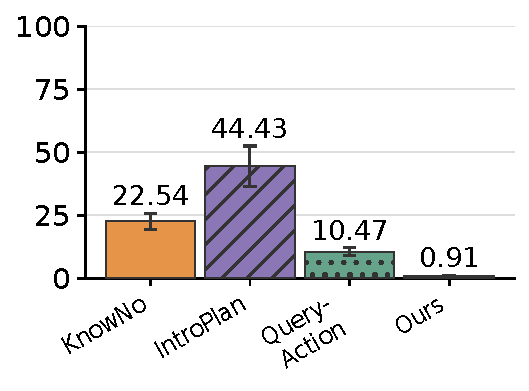
\includegraphics[width=\linewidth,height=.16\textheight,keepaspectratio]{figures/exp_oracle_waste_plan_time.pdf}
\caption{WasteSorting\\Plan time (s).}
\label{fig:baseline_oracle_waste_plan_time}
\end{subfigure}
\par\smallskip
\begin{subfigure}[t]{0.247\textwidth}
\centering
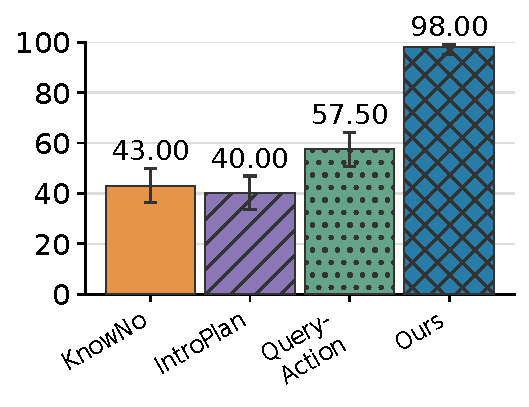
\includegraphics[width=\linewidth,height=.16\textheight,keepaspectratio]{figures/exp_oracle_tomato_success.pdf}
\caption{TomatoHarvesting\\Success rate (\%).}
\label{fig:baseline_oracle_tomato_success}
\end{subfigure}%
\hspace{0.004\textwidth}%
\begin{subfigure}[t]{0.247\textwidth}
\centering
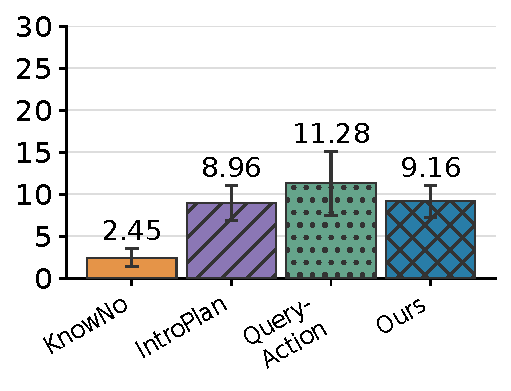
\includegraphics[width=\linewidth,height=.16\textheight,keepaspectratio]{figures/exp_oracle_tomato_queries.pdf}
\caption{TomatoHarvesting\\Query count.}
\label{fig:baseline_oracle_tomato_queries}
\end{subfigure}%
\hspace{0.004\textwidth}%
\begin{subfigure}[t]{0.247\textwidth}
\centering
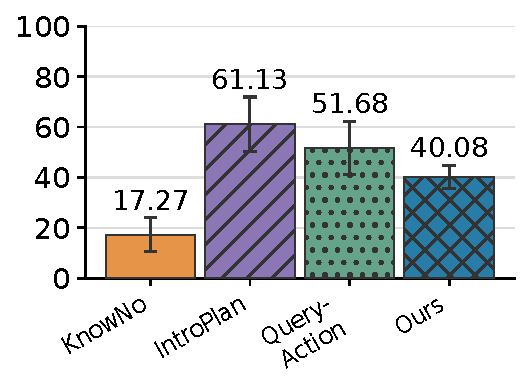
\includegraphics[width=\linewidth,height=.16\textheight,keepaspectratio]{figures/exp_oracle_tomato_query_probability.pdf}
\caption{TomatoHarvesting\\Query probability (\%).}
\label{fig:baseline_oracle_tomato_query_probability}
\end{subfigure}%
\hspace{0.004\textwidth}%
\begin{subfigure}[t]{0.247\textwidth}
\centering
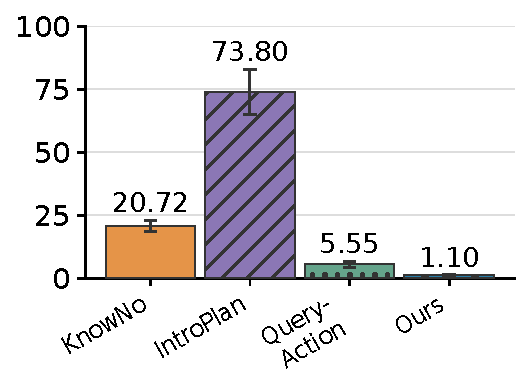
\includegraphics[width=\linewidth,height=.16\textheight,keepaspectratio]{figures/exp_oracle_tomato_plan_time.pdf}
\caption{TomatoHarvesting\\Plan time (s).}
\label{fig:baseline_oracle_tomato_plan_time}
\end{subfigure}
\caption{Oracle baseline comparison of success rate and query count and query probability and plan time. Our method achieves higher success with fewer queries and less plan time than Query-Action in both domains.}
\label{fig:baseline_results}
\end{figure*}


\begin{table*}[t]
\centering
\caption{Oracle baseline results by domain.}
\label{tab:baseline_results}
\small
\setlength{\tabcolsep}{4pt}
\begin{tabular}{llcccc}
\toprule
Domain & Method & Success (\%) & Query count & \shortstack{Query prob.(\%)} & Plan length \\
\midrule
WasteSorting & KnowNo & 48.50 & $2.48 \pm 1.42$ & $22.82 \pm 12.61$ & $10.78 \pm 1.35$ \\
 & IntroPlan & 51.50 & $6.83 \pm 1.53$ & $61.97 \pm 9.35$ & $10.99 \pm 1.49$ \\
 & Query-Action & 87.00 & $24.52 \pm 5.39$ & $87.05 \pm 5.28$ & $11.89 \pm 1.53$ \\
 & Ours & 100.00 & $7.83 \pm 2.16$ & $30.55 \pm 10.41$ & $10.35 \pm 0.88$ \\
\midrule
TomatoHarvesting & KnowNo & 43.00 & $2.45 \pm 1.06$ & $17.27 \pm 6.67$ & $14.01 \pm 1.07$ \\
 & IntroPlan & 40.00 & $8.96 \pm 2.04$ & $61.13 \pm 10.77$ & $14.61 \pm 1.46$ \\
 & Query-Action & 57.50 & $11.28 \pm 3.78$ & $51.68 \pm 10.45$ & $14.94 \pm 1.70$ \\
 & Ours & 98.00 & $9.16 \pm 1.90$ & $40.08 \pm 4.56$ & $13.97 \pm 1.15$ \\
\bottomrule
\end{tabular}
\end{table*}

As shown in Fig.~\ref{fig:baseline_results}, our method achieves the highest success rate in both domains. It completes all $200$ WasteSorting trials and $196$ of $200$ TomatoHarvesting trials. Our method achieves success rates of $100.00\%$ in WasteSorting and $98.00\%$ in TomatoHarvesting compared with $87.00\%$ and $57.50\%$ for Query-Action. The mean query counts are also lower at $7.83$ and $9.16$ compared with $24.52$ and $11.28$ for Query-Action. Two factors may explain the lower success rate and higher query count of Query-Action. First, query actions expand the action space so POMCP must evaluate more alternatives within the same simulation budget. Second, expected task reward does not explicitly measure confidence in the current state. Our method selects queries at the observation stage and restricts POMCP planning to physical actions. These results show that a higher query count alone does not guarantee a higher success rate.

Compared to KnowNo and IntroPlan, our method uses more queries. Their mean query counts are $2.48$ and $6.83$ in WasteSorting compared with $7.83$ for our method. In TomatoHarvesting, the corresponding counts are $2.45$ and $8.96$ compared with $9.16$ for our method. This difference in query count arises from how each method handles a query trigger. If a query is triggered, our method repeats queries until belief confidence reaches $\tau$. KnowNo and IntroPlan ask only one question per trigger. Therefore our method can use more queries despite a lower query probability than IntroPlan. However KnowNo and IntroPlan achieve success rates of only $48.50\%$ and $51.50\%$ in WasteSorting and $43.00\%$ and $40.00\%$ in TomatoHarvesting. Therefore a system is not necessarily better simply because it uses fewer queries.

Plan time is also lowest for Ours in both domains despite the additional queries compared with KnowNo and IntroPlan. In WasteSorting, mean plan time is $0.91$ seconds for Ours compared with $22.54$ seconds for KnowNo, $44.43$ seconds for IntroPlan, and $10.47$ seconds for Query-Action. In TomatoHarvesting, the corresponding values are $1.10$, $20.72$, $73.80$, and $5.55$ seconds. KnowNo and IntroPlan require language-model inference for candidate generation and scoring at each planning step. IntroPlan performs additional reasoning and candidate evaluation, which increases inference time compared with KnowNo. Ours evaluates query timing and selection from the belief state and searches only over physical actions. The smaller search space supports faster planning than Query-Action. The time comparisons suggest that belief-based search can reduce planning time without repeated language-model inference. % Therefore a higher query count does not necessarily imply a higher planning cost.

Our method combines confidence-based query timing with entropy gain query selection and achieves the highest success rate in both domains. The baseline comparisons suggest that effective query timing and selection are more important than query count alone.

\noindent\textbf{VLM}\label{exp:vlm_eval}. We evaluate whether the trends in task success and query behavior from the oracle experiments also hold in a real-world setting. We first prompt a VLM to act as an external expert and evaluate query policies on physical robots.\footnote{Appendix~\ref{appx:vlm_prompts} provides the VLM prompts.} We select KnowNo as the baseline because it achieves a high success rate relative to its query count in the oracle experiments. Each method has $40$ trials per domain. Figure~\ref{fig:vlm_results} presents the VLM results.

\begin{figure*}[!tp]
\centering
\begin{subfigure}[t]{0.247\textwidth}
\centering
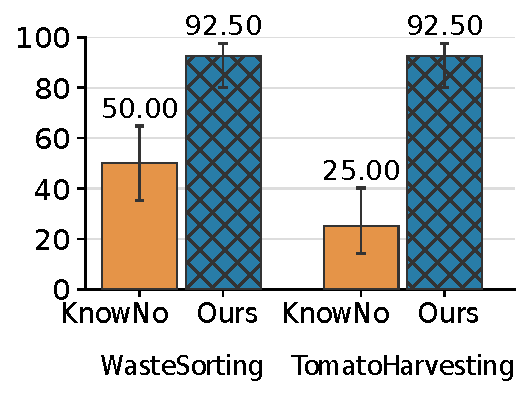
\includegraphics[width=\linewidth,height=.20\textheight,keepaspectratio]{figures/exp_vlm_success.pdf}
\caption{Success rate (\%).}
\label{fig:vlm_vlm_success}
\end{subfigure}%
\hspace{0.004\textwidth}%
\begin{subfigure}[t]{0.247\textwidth}
\centering
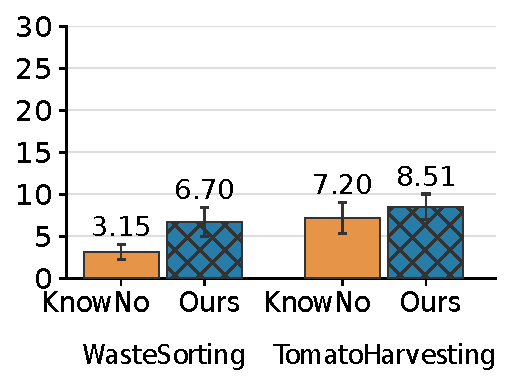
\includegraphics[width=\linewidth,height=.20\textheight,keepaspectratio]{figures/exp_vlm_queries.pdf}
\caption{Query count.}
\label{fig:vlm_vlm_queries}
\end{subfigure}%
\hspace{0.004\textwidth}%
\begin{subfigure}[t]{0.247\textwidth}
\centering
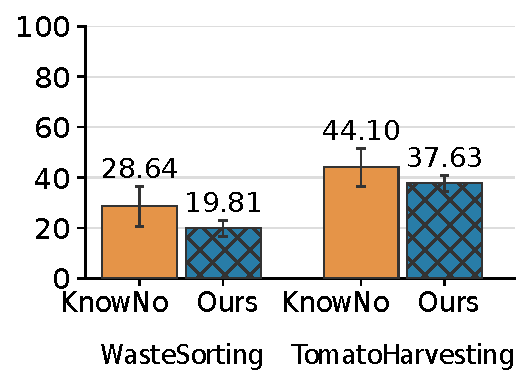
\includegraphics[width=\linewidth,height=.20\textheight,keepaspectratio]{figures/exp_vlm_query_probability.pdf}
\caption{Query probability (\%).}
\label{fig:vlm_vlm_query_probability}
\end{subfigure}%
\hspace{0.004\textwidth}%
\begin{subfigure}[t]{0.247\textwidth}
\centering
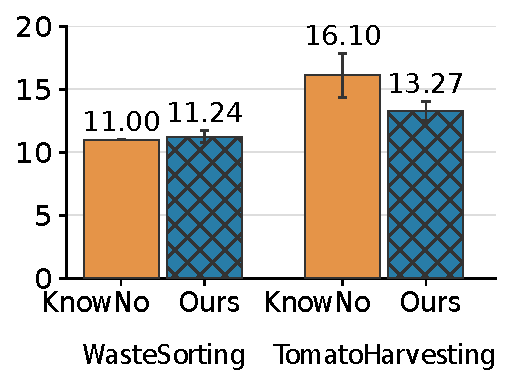
\includegraphics[width=\linewidth,height=.20\textheight,keepaspectratio]{figures/exp_vlm_plan_length.pdf}
\caption{Plan length (actions).}
\label{fig:vlm_vlm_plan_length}
\end{subfigure}
\par\smallskip
\begin{subfigure}[t]{0.247\textwidth}
\centering
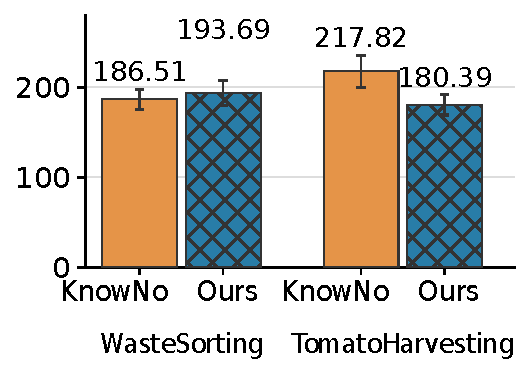
\includegraphics[width=\linewidth,height=.20\textheight,keepaspectratio]{figures/exp_vlm_total_time.pdf}
\caption{Total time (s).}
\label{fig:vlm_vlm_total_time}
\end{subfigure}%
\hspace{0.004\textwidth}%
\begin{subfigure}[t]{0.247\textwidth}
\centering
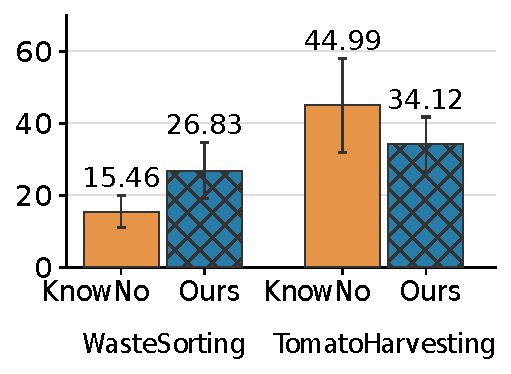
\includegraphics[width=\linewidth,height=.20\textheight,keepaspectratio]{figures/exp_vlm_interaction_time.pdf}
\caption{Interaction time (s).}
\label{fig:vlm_vlm_interaction_time}
\end{subfigure}%
\hspace{0.004\textwidth}%
\begin{subfigure}[t]{0.247\textwidth}
\centering
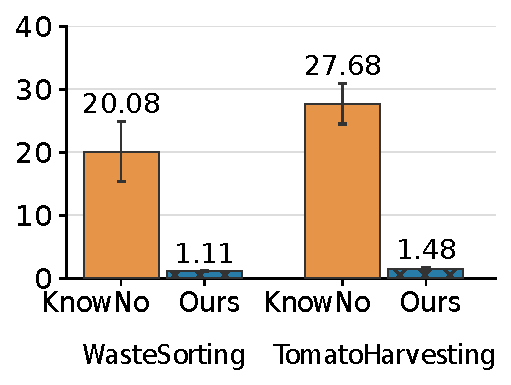
\includegraphics[width=\linewidth,height=.20\textheight,keepaspectratio]{figures/exp_vlm_planning_time.pdf}
\caption{Planning time (s).}
\label{fig:vlm_vlm_planning_time}
\end{subfigure}
\caption{Physical robot evaluation with VLM responses. Ours achieves $92.50\%$ success in both domains. Query probability is the fraction of physical steps with at least one query.}
\label{fig:vlm_results}
\end{figure*}


\begin{table*}[t]
\centering
\caption{Physical robot results with VLM and human responses. Parentheses give successful trials over all trials. Time is measured in seconds.}
\label{tab:physical_robot_results}
\small
\begin{tabular}{llccccc}
\toprule
Source & Method & Success (\%) & Queries & Total time & Interaction & Planning \\
\midrule
\multicolumn{7}{l}{WasteSorting} \\
VLM & KnowNo & 50.00 (20/40) & $3.15 \pm 0.88$ & $186.51 \pm 10.90$ & $15.46 \pm 4.45$ & $20.08 \pm 4.76$ \\
 & Ours & 92.50 (37/40) & $6.70 \pm 1.76$ & $193.69 \pm 13.52$ & $26.83 \pm 7.76$ & $1.11 \pm 0.05$ \\
Human & KnowNo & 16.67 (1/6) & $4.00 \pm \text{--}$ & $183.38 \pm \text{--}$ & $10.78 \pm \text{--}$ & $20.40 \pm \text{--}$ \\
 & Ours & 100.00 (6/6) & $6.00 \pm 1.10$ & $167.45 \pm 7.83$ & $15.65 \pm 4.90$ & $1.09 \pm 0.03$ \\
\midrule
\multicolumn{7}{l}{TomatoHarvesting} \\
VLM & KnowNo & 25.00 (10/40) & $7.20 \pm 1.87$ & $217.82 \pm 17.78$ & $44.99 \pm 13.10$ & $27.68 \pm 3.20$ \\
 & Ours & 92.50 (37/40) & $8.51 \pm 1.52$ & $180.39 \pm 11.18$ & $34.12 \pm 7.62$ & $1.48 \pm 0.19$ \\
Human & KnowNo & 33.33 (2/6) & $4.00 \pm 1.41$ & $181.89 \pm 3.38$ & $16.75 \pm 11.18$ & $25.40 \pm 3.56$ \\
 & Ours & 50.00 (3/6) & $9.67 \pm 1.53$ & $182.36 \pm 3.34$ & $27.00 \pm 2.64$ & $1.46 \pm 0.13$ \\
\bottomrule
\end{tabular}
\end{table*}

Ours achieves a success rate of $92.50\%$ in both domains with VLM responses. KnowNo achieves $50.00\%$ in WasteSorting and $25.00\%$ in TomatoHarvesting. Mean query counts are $6.70$ for Ours and $3.15$ for KnowNo in WasteSorting and $8.51$ and $7.20$ in TomatoHarvesting. Consistent with the oracle experiments, Ours requires less search time than KnowNo. Mean search time is $0.99$ seconds for Ours and $19.99$ seconds for KnowNo in WasteSorting and $1.38$ and $26.90$ seconds in TomatoHarvesting. In TomatoHarvesting, interaction time and total time are $44.99$ and $217.82$ seconds for KnowNo compared with $34.12$ and $180.39$ seconds for Ours. Notably, KnowNo uses only $15.43\%$ fewer queries than Ours in TomatoHarvesting with VLM responses compared with $73.22\%$ fewer queries in the oracle experiments. However the similar query counts do not translate into similar execution costs. KnowNo executes longer plans, with $16.10$ physical actions compared with $13.27$ for Ours. Interaction time and total time for KnowNo are $31.86\%$ and $20.75\%$ longer than for Ours respectively.

To understand the differences from the oracle results, we analyze failed trials and distinguish VLM response errors from baseline planner failures. In WasteSorting, all three failures of Ours involve VLM feedback. For example, the VLM rejects a can classification from perception and the robot places the object in the plastic bin. KnowNo has three VLM response failures ($15\%$) and $17$ planner failures ($85\%$). The planner failures occur because KnowNo selects actions without requesting assistance despite unmet action preconditions. In TomatoHarvesting, all three failures of Ours also involve VLM feedback. KnowNo has $18$ VLM failures ($60\%$) and $12$ planner failures ($40\%$). The planner failures occur after action selections without external assistance. In six trials, the VLM repeatedly selects detection despite feasible alternatives and the robot reaches the step limit. The remaining $12$ VLM failures involve incorrect action selections.

The WasteSorting failures show that a single predicted action can still require additional state verification before execution. In TomatoHarvesting, action selection requires the VLM to reason about robot location and object states to determine the next action. The spatial reasoning burden can lead to less effective action choices. Even successful trials can then require additional queries and longer plans and more total time. Therefore fewer queries do not necessarily reduce interaction time or total time. Ours asks the VLM to verify current state facts and assigns action selection to the planner. The VLM assesses current observations with less need to reason about future actions and outcomes. Performance may also depend on what the VLM is asked to judge.

\noindent\textbf{Human}\label{exp:human_eval}. We further examine whether the trends in task success and query behavior persist with human feedback. We provide five participants with domain information including the task goals and available actions. \textit{The provisional participant profile assumes two men and three women with a mean age of approximately $25$ years and an age range of $20$--$30$ years. These demographic values are placeholders and are not yet verified.} Participants use the tablet interface in Fig.~\ref{fig:human_tablet_interface} to answer robot questions. Participants choose responses based on their own judgment. We use the same robot platforms and task domains as in the VLM experiments. Each method has $10$ trials per domain. Figure~\ref{fig:human_results} presents the human evaluation results. Table~\ref{tab:physical_robot_results} reports the results of both the VLM and human evaluations.
% Replace the provisional demographics after participant data collection.


% Update the numerical results after the five-participant evaluation. Current values use six trials per domain and method.
% Planning times use the successful-trial values provided in the human experiment table.
Ours achieves a success rate of $100.00\%$ in WasteSorting and $50.00\%$ in TomatoHarvesting with human responses. KnowNo achieves $16.67\%$ and $33.33\%$ respectively. Mean query counts are $6.00$ for Ours and $4.00$ for KnowNo in WasteSorting and $9.67$ and $4.00$ in TomatoHarvesting. Mean planning time is $1.09$ seconds for Ours and $20.40$ seconds for KnowNo in WasteSorting and $1.46$ and $25.40$ seconds in TomatoHarvesting. In WasteSorting, interaction time and total time are $15.65$ and $167.45$ seconds for Ours compared with $10.78$ and $183.38$ seconds for KnowNo. In TomatoHarvesting, the corresponding times are $27.00$ and $182.36$ seconds for Ours compared with $16.75$ and $181.89$ seconds for KnowNo. KnowNo uses $33.33\%$ fewer queries than Ours in WasteSorting and $58.62\%$ fewer in TomatoHarvesting. However the lower query counts do not consistently reduce total time. Plan lengths are similar across methods, with $11.00$ physical actions for both methods in WasteSorting and $13.33$ for Ours and $13.00$ for KnowNo in TomatoHarvesting. Despite the additional queries, Ours requires $8.69\%$ less total time in WasteSorting and a similar total time in TomatoHarvesting.

\noindent\textbf{Comparison Across Feedback Sources}\label{exp:response_comparison}. Figure~\ref{fig:response_comparison} compares task success and query count across oracle, VLM, and human feedback. Ours achieves higher success rates and uses more queries than KnowNo in both domains across all three feedback sources. However the magnitude of the success advantage depends on the domain and feedback source. In WasteSorting, Ours maintains success rates of $100.00\%$, $92.50\%$, and $100.00\%$ with oracle, VLM, and human feedback respectively. In TomatoHarvesting, success decreases from $98.00\%$ with oracle feedback to $92.50\%$ with VLM feedback and $50.00\%$ with human feedback. The success advantage over KnowNo also narrows from $55.00$ percentage points with oracle feedback to $16.67$ percentage points with human feedback in TomatoHarvesting. Thus the relative advantage of Ours persists, but high success does not persist equally across domains and feedback sources.

Query counts also show differences across feedback sources. In TomatoHarvesting, Ours uses $9.16$, $8.51$, and $9.67$ queries with oracle, VLM, and human feedback respectively. KnowNo uses $2.45$, $7.20$, and $4.00$ queries. The query count of KnowNo increases substantially with VLM feedback, while the query count of Ours remains similar across feedback sources despite the lower success with human feedback. Therefore similar query counts do not imply similar task outcomes, and the number of queries alone does not explain the differences across feedback sources. These differences motivate the subsequent human interview analysis. We examine how participants interpret robot questions and what reasoning participants need to choose a response, with particular attention to question clarity and response effort.


\begin{figure}[t]
\centering
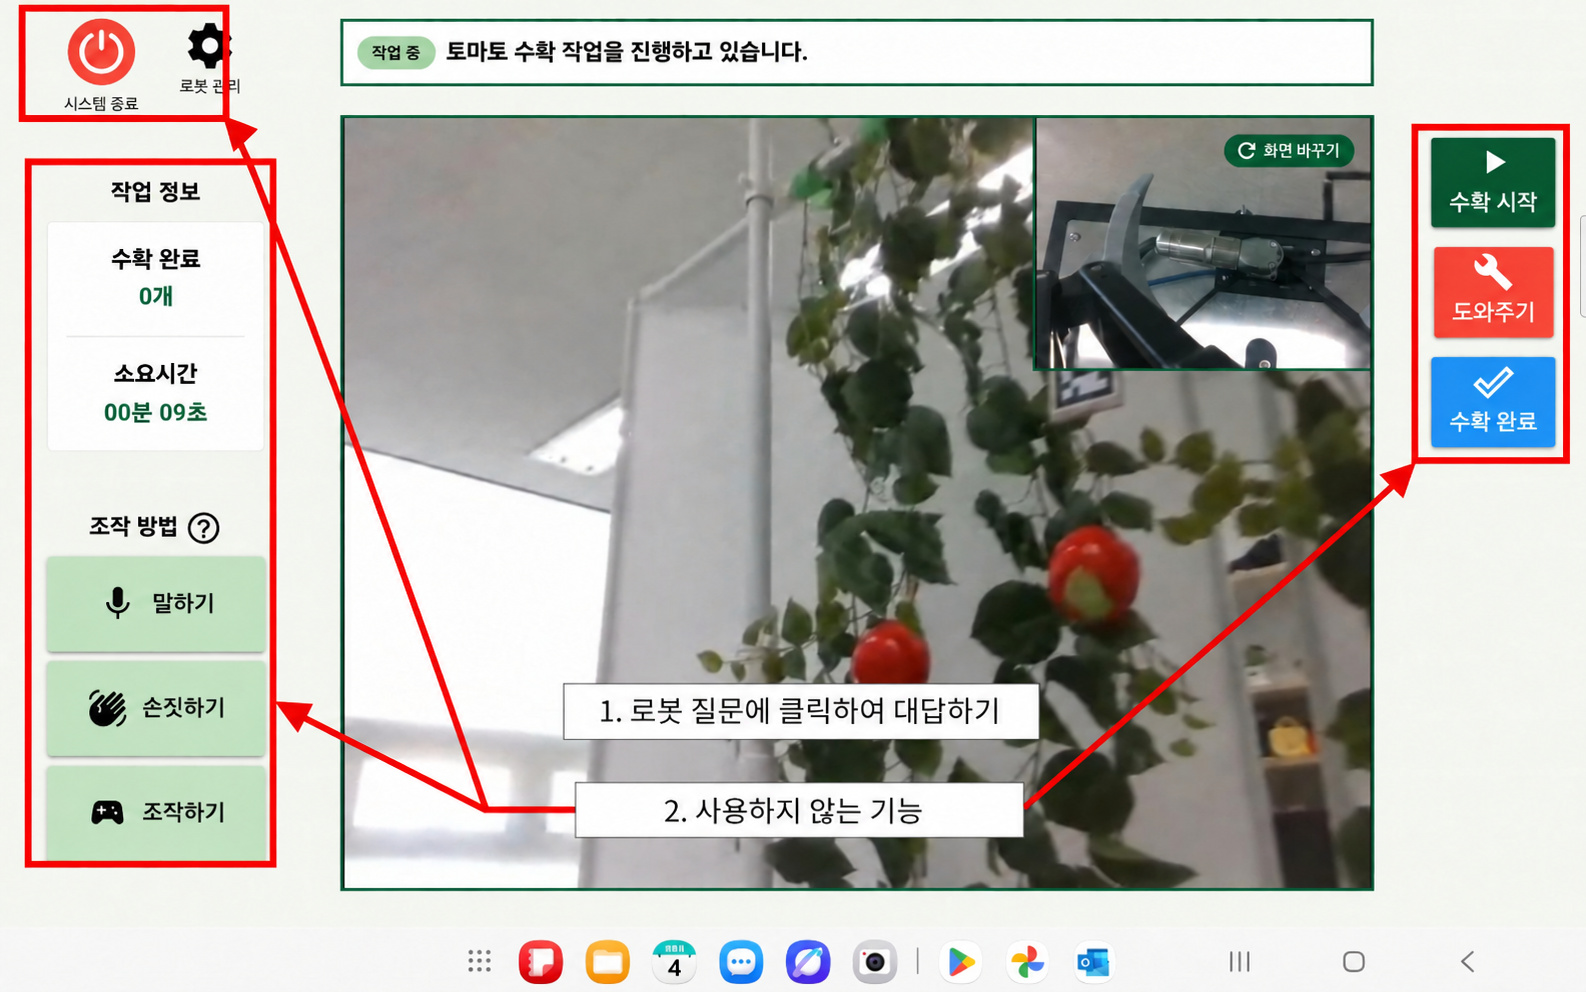
\includegraphics[width=\linewidth]{figures/human_tablet_interface.jpg}
\caption{Tablet interface used in the human evaluation. Participants view the robot camera feeds and select responses to robot queries.}
\label{fig:human_tablet_interface}
\end{figure}

\begin{figure*}[!tp]
\centering
\begin{subfigure}[t]{0.247\textwidth}
\centering
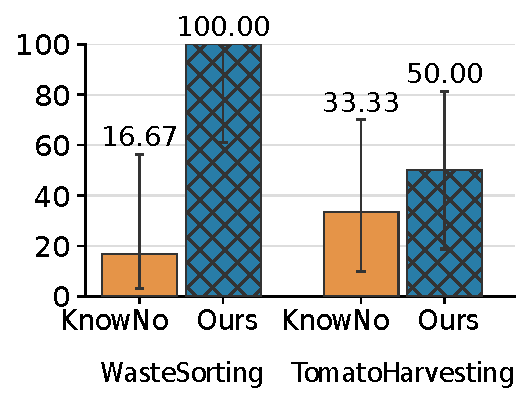
\includegraphics[width=\linewidth,height=.20\textheight,keepaspectratio]{figures/exp_human_success.pdf}
\caption{Success rate (\%).}
\label{fig:human_human_success}
\end{subfigure}%
\hspace{0.004\textwidth}%
\begin{subfigure}[t]{0.247\textwidth}
\centering
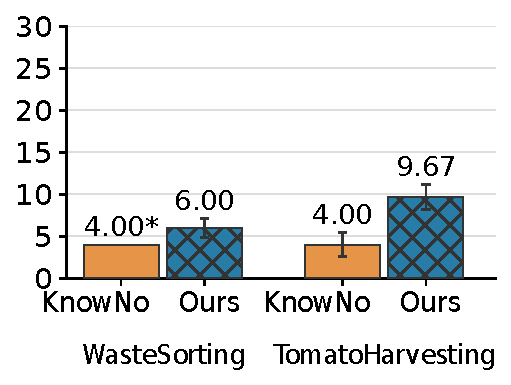
\includegraphics[width=\linewidth,height=.20\textheight,keepaspectratio]{figures/exp_human_queries.pdf}
\caption{Query count.}
\label{fig:human_human_queries}
\end{subfigure}%
\hspace{0.004\textwidth}%
\begin{subfigure}[t]{0.247\textwidth}
\centering
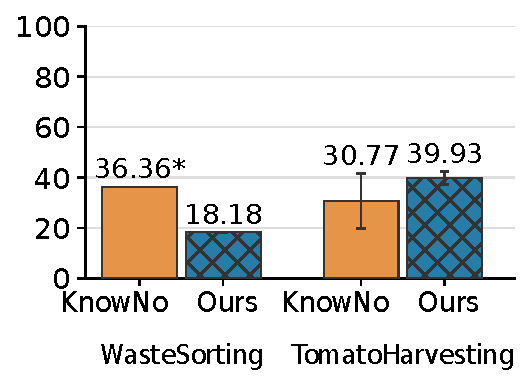
\includegraphics[width=\linewidth,height=.20\textheight,keepaspectratio]{figures/exp_human_query_probability.pdf}
\caption{Query probability (\%).}
\label{fig:human_human_query_probability}
\end{subfigure}%
\hspace{0.004\textwidth}%
\begin{subfigure}[t]{0.247\textwidth}
\centering
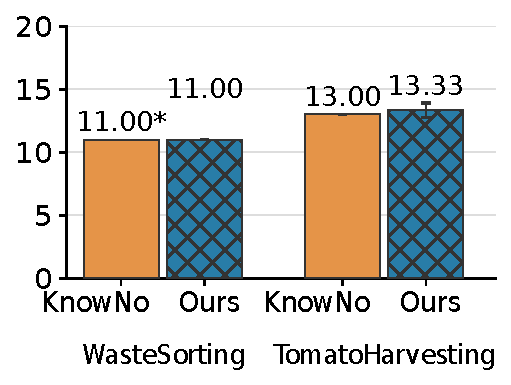
\includegraphics[width=\linewidth,height=.20\textheight,keepaspectratio]{figures/exp_human_plan_length.pdf}
\caption{Plan length (actions).}
\label{fig:human_human_plan_length}
\end{subfigure}
\par\smallskip
\begin{subfigure}[t]{0.247\textwidth}
\centering
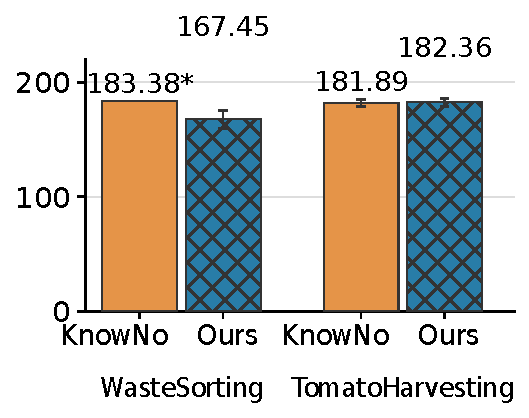
\includegraphics[width=\linewidth,height=.20\textheight,keepaspectratio]{figures/exp_human_total_time.pdf}
\caption{Total time (s).}
\label{fig:human_human_total_time}
\end{subfigure}%
\hspace{0.004\textwidth}%
\begin{subfigure}[t]{0.247\textwidth}
\centering
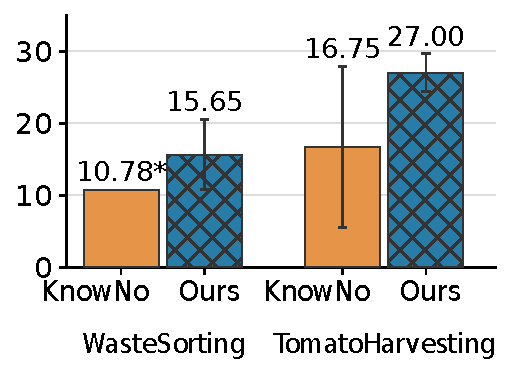
\includegraphics[width=\linewidth,height=.20\textheight,keepaspectratio]{figures/exp_human_interaction_time.pdf}
\caption{Interaction time (s).}
\label{fig:human_human_interaction_time}
\end{subfigure}%
\hspace{0.004\textwidth}%
\begin{subfigure}[t]{0.247\textwidth}
\centering
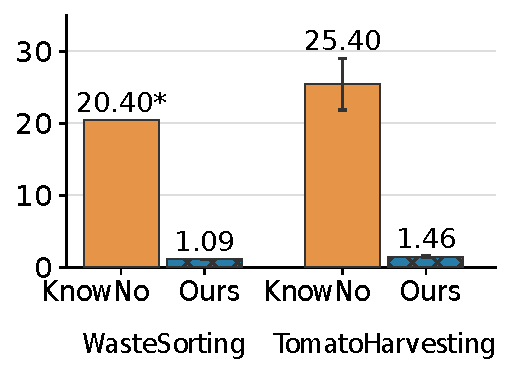
\includegraphics[width=\linewidth,height=.20\textheight,keepaspectratio]{figures/exp_human_planning_time.pdf}
\caption{Planning time (s).}
\label{fig:human_human_planning_time}
\end{subfigure}
\caption{Physical robot evaluation with human responses. Ours completes six WasteSorting trials and three TomatoHarvesting trials. An asterisk denotes a single successful trial with no sample standard deviation.}
\label{fig:human_results}
\end{figure*}

\begin{figure*}[!tp]
\centering
\begin{subfigure}[t]{0.495\textwidth}
\centering
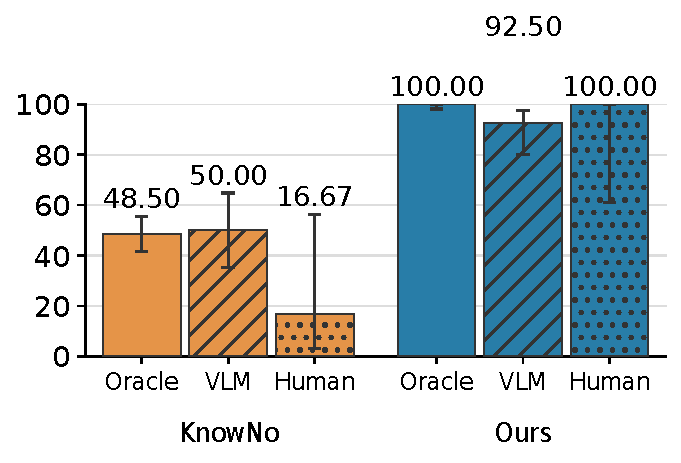
\includegraphics[width=\linewidth,height=.20\textheight,keepaspectratio]{figures/exp_response_waste_success.pdf}
\caption{WasteSorting. Success rate (\%).}
\label{fig:response_response_waste_success}
\end{subfigure}
\hfill
\begin{subfigure}[t]{0.495\textwidth}
\centering
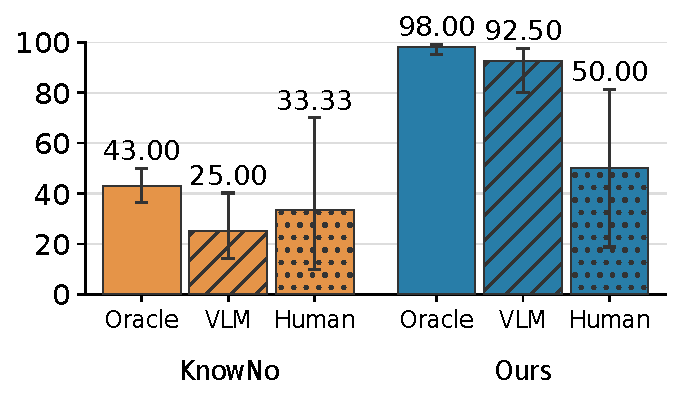
\includegraphics[width=\linewidth,height=.20\textheight,keepaspectratio]{figures/exp_response_tomato_success.pdf}
\caption{TomatoHarvesting. Success rate (\%).}
\label{fig:response_response_tomato_success}
\end{subfigure}
\par\medskip
\begin{subfigure}[t]{0.495\textwidth}
\centering
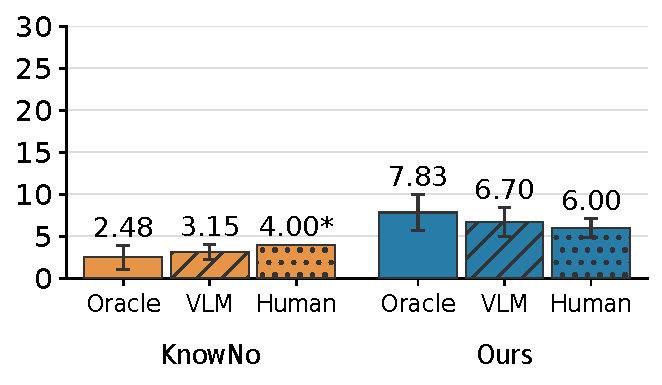
\includegraphics[width=\linewidth,height=.20\textheight,keepaspectratio]{figures/exp_response_waste_queries.pdf}
\caption{WasteSorting. Query count.}
\label{fig:response_response_waste_queries}
\end{subfigure}
\hfill
\begin{subfigure}[t]{0.495\textwidth}
\centering
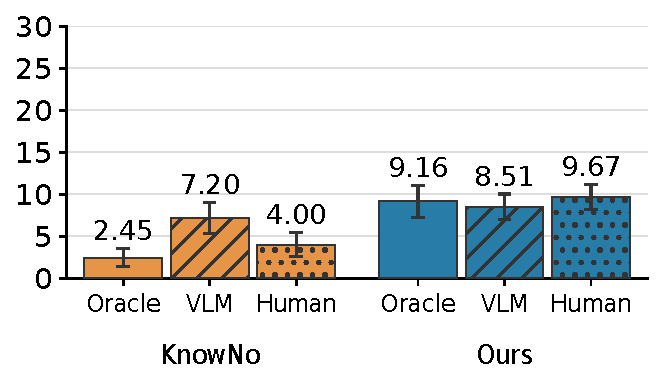
\includegraphics[width=\linewidth,height=.20\textheight,keepaspectratio]{figures/exp_response_tomato_queries.pdf}
\caption{TomatoHarvesting. Query count.}
\label{fig:response_response_tomato_queries}
\end{subfigure}
\caption{Comparison of oracle simulation and physical execution with VLM and human responses. Each response condition retains its own trial set.}
\label{fig:response_comparison}
\end{figure*}





\subsubsection{Ablation Study}~\label{exp:when_what_random}\label{exp:policy_ablation}

We conduct an ablation study to assess the contributions of query timing and query selection to task success and query efficiency. We compare seven configurations with oracle feedback in simulation. For concise reference, we use \textbf{W} to label query timing variants and \textbf{Q} to label query selection variants. With entropy gain selection fixed, we compare random (W1), conformal prediction (W2), and reward-based (W3) timing. With confidence timing fixed, we compare random (Q1) and reward-based (Q2) selection. Fully-Random randomizes both query timing and query selection, while Ours combines confidence timing with entropy gain selection. Table~\ref{tab:query_strategy_matrix} summarizes these configurations. Each configuration has $200$ trials per domain. Table~\ref{tab:policy_ablation} and Fig.~\ref{fig:policy_ablation_results} present the results. Appendix~\ref{appx:ablation_configs} provides the query policy configurations.

\begin{figure*}[!tp]
\centering
\begin{subfigure}[t]{0.495\textwidth}
\centering
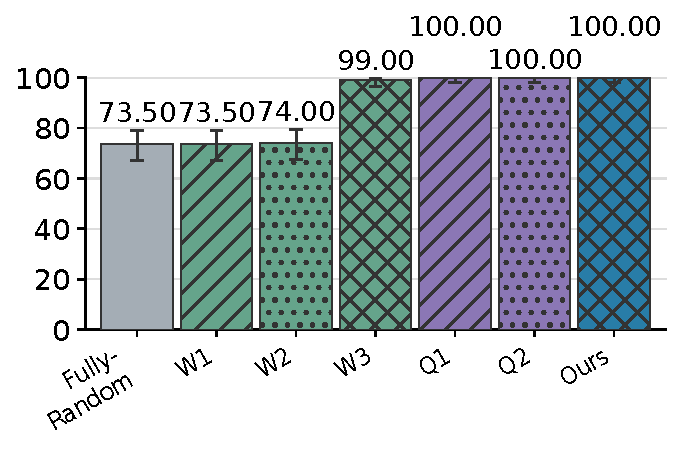
\includegraphics[width=\linewidth,height=.20\textheight,keepaspectratio]{figures/exp_ablation_waste_success.pdf}
\caption{WasteSorting. Success rate (\%).}
\label{fig:ablation_ablation_waste_success}
\end{subfigure}
\hfill
\begin{subfigure}[t]{0.495\textwidth}
\centering
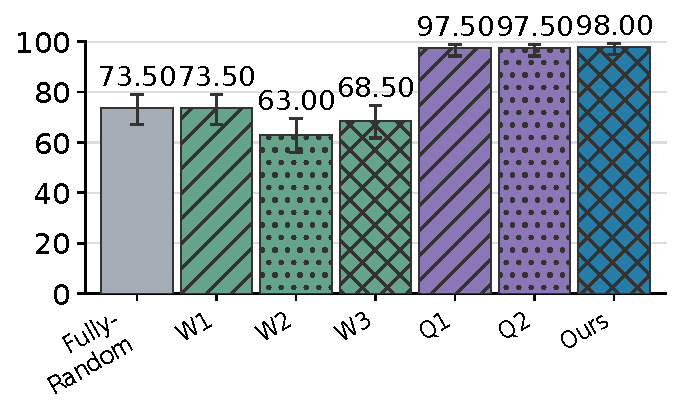
\includegraphics[width=\linewidth,height=.20\textheight,keepaspectratio]{figures/exp_ablation_tomato_success.pdf}
\caption{TomatoHarvesting. Success rate (\%).}
\label{fig:ablation_ablation_tomato_success}
\end{subfigure}
\par\medskip
\begin{subfigure}[t]{0.495\textwidth}
\centering
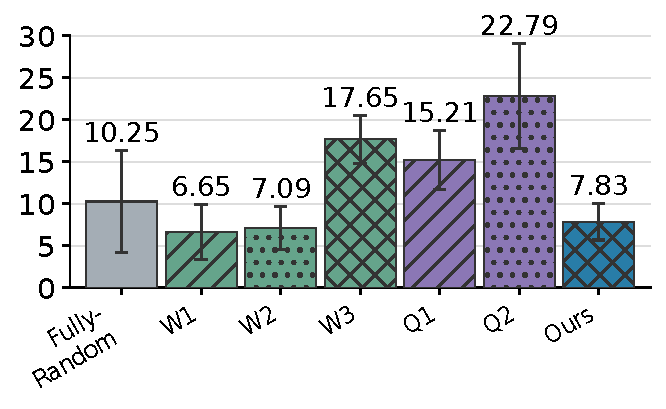
\includegraphics[width=\linewidth,height=.20\textheight,keepaspectratio]{figures/exp_ablation_waste_queries.pdf}
\caption{WasteSorting. Query count.}
\label{fig:ablation_ablation_waste_queries}
\end{subfigure}
\hfill
\begin{subfigure}[t]{0.495\textwidth}
\centering
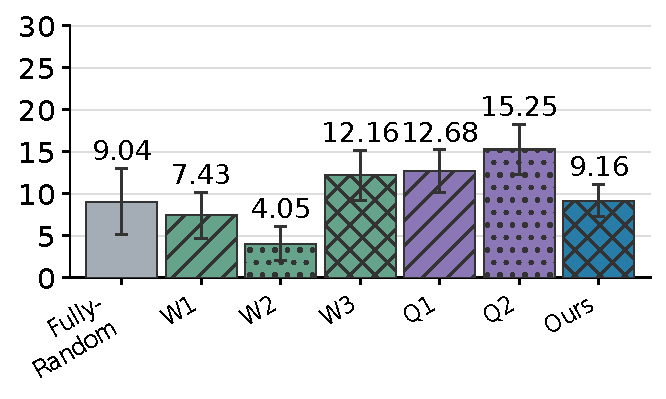
\includegraphics[width=\linewidth,height=.20\textheight,keepaspectratio]{figures/exp_ablation_tomato_queries.pdf}
\caption{TomatoHarvesting. Query count.}
\label{fig:ablation_ablation_tomato_queries}
\end{subfigure}
\caption{Query timing and selection ablation. W1--W3 vary query timing and Q1--Q2 vary query selection. Confidence timing supports high success, and entropy gain selection reduces query count at similar success rates.}
\label{fig:policy_ablation_results}
\end{figure*}


\begin{table*}[t]
\centering
\caption{Query policy ablation. W1--W3 compare timing criteria and Q1--Q2 compare selection criteria.}
\label{tab:policy_ablation}
\label{tab:when_what_random}
\small
\setlength{\tabcolsep}{4pt}
\begin{tabular}{lllcccc}
\toprule
 & & & \multicolumn{2}{c}{WasteSorting} & \multicolumn{2}{c}{TomatoHarvesting} \\
\cmidrule(lr){4-5}\cmidrule(lr){6-7}
Condition & Timing & Selection & Success (\%) & Queries & Success (\%) & Queries \\
\midrule
Fully-Random & Random & Random & 73.50 & $10.25 \pm 6.11$ & 73.50 & $9.04 \pm 3.94$ \\
W1 & Random & Entropy Gain & 73.50 & $6.65 \pm 3.29$ & 73.50 & $7.43 \pm 2.72$ \\
W2 & Conformal Prediction & Entropy Gain & 74.00 & $7.09 \pm 2.58$ & 63.00 & $4.05 \pm 2.04$ \\
W3 & Reward & Entropy Gain & 99.00 & $17.65 \pm 2.89$ & 68.50 & $12.16 \pm 3.00$ \\
Q1 & Confidence & Random & 100.00 & $15.21 \pm 3.53$ & 97.50 & $12.68 \pm 2.53$ \\
Q2 & Confidence & Reward & 100.00 & $22.79 \pm 6.26$ & 97.50 & $15.25 \pm 2.95$ \\
Ours & Confidence & Entropy Gain & 100.00 & $7.83 \pm 2.16$ & 98.00 & $9.16 \pm 1.90$ \\
\bottomrule
\end{tabular}
\end{table*}

The timing comparison evaluates Fully-Random, W1--W3, and Ours. In WasteSorting, Fully-Random and W1 achieve $73.50\%$ success, and W2 achieves $74.00\%$. W3 achieves $99.00\%$ compared with $100.00\%$ for Ours, but requires $17.65$ queries compared with $7.83$. Fully-Random, W1, and W2 use $10.25$, $6.65$, and $7.09$ queries respectively. In TomatoHarvesting, Fully-Random and W1 achieve $73.50\%$ success, while W2 and W3 achieve $63.00\%$ and $68.50\%$ compared with $98.00\%$ for Ours. Mean query counts are $9.04$ for Fully-Random, $7.43$ for W1, $4.05$ for W2, $12.16$ for W3, and $9.16$ for Ours.

These results show that task success depends on the query trigger as well as query selection. W1 replaces random selection in Fully-Random with entropy gain and reduces query count without improving success. Random timing can miss necessary verification because the trigger does not depend on current state uncertainty. W2 can also end queries after the action prediction set narrows to one candidate, even if the state facts required to execute the candidate action remain uncertain. W3 uses expected task reward to determine whether to initiate queries, then selects queries by entropy gain and repeats verification until confidence reaches $\tau$. In WasteSorting, object category verification directly informs the correct bin choice and task reward, so repeated verification may support the high success rate of $99.00\%$. However W3 requires $125.43\%$ more queries than Ours. In TomatoHarvesting, W3 uses $32.71\%$ more queries than Ours, but the success rate of W3 is $29.50$ percentage points lower. Therefore reward-based timing can request more queries overall and still fail to verify necessary state information at the appropriate time. Thus Ours uses current state confidence as the query trigger and achieves the highest success in both domains with fewer queries than reward-based timing.

With confidence-based query timing fixed, different query selection strategies maintain high success rates but require different numbers of queries. The query selection comparison evaluates Fully-Random, Q1, Q2, and Ours. Fully-Random achieves $73.50\%$ success in both domains with $10.25$ queries in WasteSorting and $9.04$ in TomatoHarvesting. Q1 retains random selection but uses confidence timing, and success increases to $100.00\%$ and $97.50\%$ respectively. With confidence timing fixed, Q1, Q2, and Ours all achieve $100.00\%$ success in WasteSorting. Mean query counts are $15.21$ for Q1, $22.79$ for Q2, and $7.83$ for Ours. In TomatoHarvesting, Q1 and Q2 achieve $97.50\%$ success compared with $98.00\%$ for Ours. Mean query counts are $12.68$ for Q1, $15.25$ for Q2, and $9.16$ for Ours.

Confidence timing maintains $100.00\%$ success in WasteSorting and at least $97.50\%$ in TomatoHarvesting across all three query selection strategies. Under confidence timing, query selection primarily affects the number of queries needed to reach the required confidence. Random selection does not prioritize facts by their expected reduction in state uncertainty. Reward-based selection evaluates expected task reward without directly measuring the information provided by a query response. Entropy gain selects facts according to the expected reduction in state uncertainty, so the selection criterion matches the confidence requirement that ends a query episode. Relative to Q1 and Q2, Ours reduces query count by $48.54\%$ and $65.64\%$ in WasteSorting and by $27.72\%$ and $39.92\%$ in TomatoHarvesting. Thus our query selection method reduces the number of queries required under confidence timing without reducing task success.

These results support the main contribution of our method through the distinct roles of query timing and query selection. Query timing determines whether the robot requests additional information before it executes actions under state uncertainty. Confidence timing achieves high success with random, reward-based, and entropy gain selection, while entropy gain under random timing reduces query count without improving success over Fully-Random. Once confidence timing establishes a high success level, entropy gain reduces the number of queries needed to reach the required confidence. Therefore our method combines a timing criterion that supports task success with a selection criterion that reduces query count at that success level.

\subsubsection{Threshold Experiments}~\label{exp:sys_threshold}

After the ablation comparison, we examine how the confidence threshold controls task success and query count. We vary $\tau$ from $0.0$ to $1.0$ in increments of $0.1$ with entropy gain selection fixed and correct oracle responses in simulation. Each threshold has $200$ trials per domain. Table~\ref{tab:threshold_results} and Fig.~\ref{fig:threshold_results} present the results. The results at $\tau=0.8$ use the same Ours trials as the baseline and ablation comparisons, as specified in Appendix~\ref{appx:oracle_reference}.

\begin{figure*}[!tp]
\centering
\begin{subfigure}[t]{0.49\textwidth}
\centering
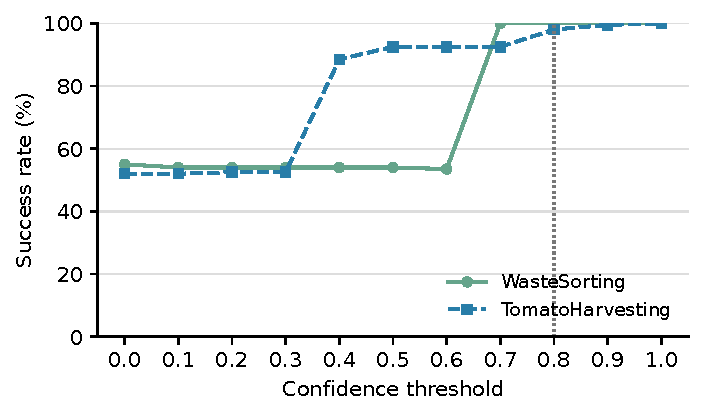
\includegraphics[width=\linewidth]{figures/exp_threshold_success.pdf}
\caption{Task success.}
\label{fig:threshold_success}
\end{subfigure}
\hfill
\begin{subfigure}[t]{0.49\textwidth}
\centering
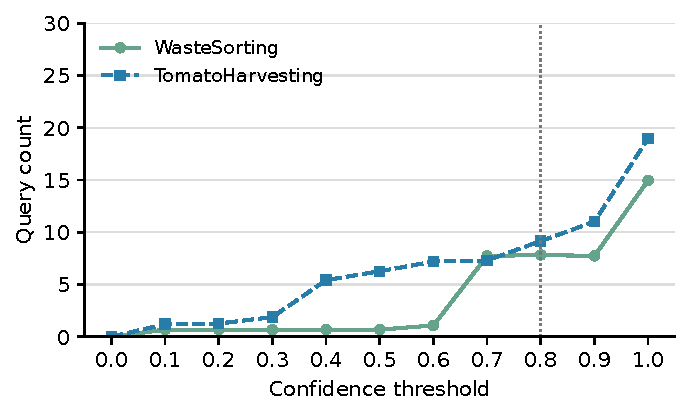
\includegraphics[width=\linewidth]{figures/exp_threshold_queries.pdf}
\caption{Mean query count.}
\label{fig:threshold_queries}
\end{subfigure}
\caption{Effect of the confidence threshold on task success and query count. The dotted line marks the default threshold of $\tau=0.8$. Requiring confidence of $1.0$ substantially increases query count with little or no additional success.}
\label{fig:threshold_results}
\end{figure*}


\begin{table*}[t]
\centering
\caption{Task success and query count across confidence thresholds.}
\label{tab:threshold_results}
\small
\begin{tabular}{ccccc}
\toprule
 & \multicolumn{2}{c}{WasteSorting} & \multicolumn{2}{c}{TomatoHarvesting} \\
\cmidrule(lr){2-3}\cmidrule(lr){4-5}
$\tau$ & Success (\%) & Queries & Success (\%) & Queries \\
\midrule
0.0 & 55.00 & $0.00 \pm 0.00$ & 52.00 & $0.00 \pm 0.00$ \\
0.1 & 54.00 & $0.69 \pm 0.84$ & 52.00 & $1.21 \pm 1.43$ \\
0.2 & 54.00 & $0.69 \pm 0.84$ & 52.50 & $1.27 \pm 1.42$ \\
0.3 & 54.00 & $0.69 \pm 0.84$ & 52.50 & $1.89 \pm 1.83$ \\
0.4 & 54.00 & $0.69 \pm 0.84$ & 88.50 & $5.42 \pm 2.30$ \\
0.5 & 54.00 & $0.69 \pm 0.84$ & 92.50 & $6.27 \pm 2.07$ \\
0.6 & 53.50 & $1.08 \pm 0.97$ & 92.50 & $7.20 \pm 1.99$ \\
0.7 & 100.00 & $7.74 \pm 2.25$ & 92.50 & $7.30 \pm 2.04$ \\
0.8 & 100.00 & $7.83 \pm 2.16$ & 98.00 & $9.16 \pm 1.90$ \\
0.9 & 100.00 & $7.74 \pm 2.25$ & 99.50 & $11.02 \pm 1.52$ \\
1.0 & 100.00 & $14.97 \pm 2.02$ & 100.00 & $19.00 \pm 1.43$ \\
\bottomrule
\end{tabular}
\end{table*}

In WasteSorting, success improves sharply at $\tau=0.7$ and remains constant at higher thresholds. With $\tau=0.0$, the robot makes no queries and achieves $55.00\%$ success. Thresholds from $0.1$ to $0.6$ yield success rates between $53.50\%$ and $54.00\%$ with at most $1.08$ queries on average. At $\tau=0.7$, success reaches $100.00\%$ with $7.74$ queries. Success remains $100.00\%$ over $\tau=0.7$--$0.9$, and query count stays between $7.74$ and $7.83$. However $\tau=1.0$ requires $14.97$ queries without further success improvement. The additional queries confirm that the strictest confidence requirement can increase interaction frequency after task success reaches its maximum.

In TomatoHarvesting, higher thresholds improve success over a wider range. Success is $52.00\%$ without queries at $\tau=0.0$ and remains at most $52.50\%$ through $\tau=0.3$. At $\tau=0.4$, success increases to $88.50\%$ with $5.42$ queries. Success reaches $92.50\%$ over $\tau=0.5$--$0.7$ and $98.00\%$ at $\tau=0.8$ with $9.16$ queries. Raising $\tau$ to $0.9$ increases success to $99.50\%$ with $11.02$ queries. At $\tau=1.0$, success reaches $100.00\%$ with $19.00$ queries. Therefore the increase from $0.9$ to $1.0$ adds $7.98$ queries for only $0.50$ percentage points of additional success.

The two domains require different confidence levels to reach high success, but both show limited gains from the strictest threshold. Relative to $\tau=0.8$, $\tau=1.0$ increases query count by $91.19\%$ in WasteSorting and $107.30\%$ in TomatoHarvesting. Success improves by $0.00$ and $2.00$ percentage points respectively. We use $\tau=0.8$ as a common threshold because it achieves $100.00\%$ and $98.00\%$ success in the two domains with substantially fewer queries than $\tau=1.0$. Thus the threshold controls the amount of state verification, and the highest confidence requirement does not provide a proportional improvement in task success.

\subsubsection*{Interviews}\label{exp:interviews}

% Interview protocol and analyzed findings remain to be adds.
% Address comprehension of state verification and action selection questions.
% Report participant evidence about reasoning effort and repeated requests.

\subsubsection*{Discussion}\label{exp:discussion}

The experiments show that query timing and query selection make distinct contributions to successful task execution. Confidence timing maintains success rates close to $100\%$ across random, reward-based, and entropy gain selection in the oracle experiments. Entropy gain reduces the number of queries required at that success level. The Fully-Random and W1 comparison further shows that effective selection alone does not recover high success if query timing remains random. The threshold experiments also show that stricter state verification increases query count without a proportional improvement in success. Together, these results support the separation of a timing criterion that identifies the need for state information from a selection criterion that reduces the cost of obtaining sufficient information.

Physical execution with VLM feedback preserves the success advantage of Ours, but additional queries have different effects on execution time across domains. Ours uses more queries than KnowNo in both domains, while total time is longer in WasteSorting and shorter in TomatoHarvesting. In TomatoHarvesting, KnowNo uses nearly as many queries as Ours but executes longer plans and requires more interaction time. The failure analysis also identifies action choices that are feasible but do not advance the task. Action selection requires the VLM to reason about robot location and object states to determine the next action. Ours asks the VLM to verify current state facts and leaves action selection to the planner. Therefore execution cost depends on the judgments required from the feedback source and the subsequent actions, as well as the number of queries.

% Provisional interview interpretation. This paragraph states hypotheses and must be revised using participant interview evidence.
The query format may also affect the effort required to provide human feedback. State verification gives participants a specific fact to assess from the current observations. Action selection requires participants to compare alternatives and consider how the next action contributes to the task goal. Therefore participants may find frequent state verification questions easier to answer than fewer action selection questions. Repeated verification can still interrupt the task or become burdensome if the purpose of each question is unclear. These possible responses suggest that question clarity and the reasoning required for each answer matter alongside query frequency. The participant interviews examine whether the differences in required judgment also appear in the perceived interaction effort.

% % Keep the experimental figures and tables before the conclusion.
% \clearpage
